%%%%%%%%%%%%%%%%%%%%%%%%%%%%%%%%%%%%%
%                                   %
% Compile with XeLaTeX and biber    %
%                                   %
% Questions or comments:            %
%                                   %
% joshua dot mcneill at uga dot edu %
%                                   %
%%%%%%%%%%%%%%%%%%%%%%%%%%%%%%%%%%%%%

\documentclass{beamer}
  % Read in standard preamble (cosmetic stuff)
  %%%%%%%%%%%%%%%%%%%%%%%%%%%%%%%%%%%%%%%%%%%%%%%%%%%%%%%%%%%%%%%%
% This is a standard preamble used in for all slide documents. %
% It basically contains cosmetic settings.                     %
%                                                              %
% Joshua McNeill                                               %
% joshua dot mcneill at uga dot edu                            %
%%%%%%%%%%%%%%%%%%%%%%%%%%%%%%%%%%%%%%%%%%%%%%%%%%%%%%%%%%%%%%%%

% Beamer settings
% \usetheme{Berkeley}
\usetheme{CambridgeUS}
% \usecolortheme{dove}
% \usecolortheme{rose}
\usecolortheme{seagull}
\usefonttheme{professionalfonts}
\usefonttheme{serif}
\setbeamertemplate{bibliography item}{}

% Packages and settings
\usepackage{fontspec}
  \setmainfont{Charis SIL}
\usepackage{hyperref}
  \hypersetup{colorlinks=true,
              allcolors=blue}
\usepackage{graphicx}
  \graphicspath{{../../figures/}}
\usepackage[normalem]{ulem}
\usepackage{enumerate}

% Document information
\author{M. McNeill}
\title[FREN2001]{Français 2001}
\institute{\url{joshua.mcneill@uga.edu}}
\date{}

%% Custom commands
% Lexical items
\newcommand{\lexi}[1]{\textit{#1}}
% Gloss
\newcommand{\gloss}[1]{`#1'}
\newcommand{\tinygloss}[1]{{\tiny`#1'}}
% Orthographic representations
\newcommand{\orth}[1]{$\langle$#1$\rangle$}
% Utterances (pragmatics)
\newcommand{\uttr}[1]{`#1'}
% Sentences (pragmatics)
\newcommand{\sent}[1]{\textit{#1}}
% Base dir for definitions
\newcommand{\defs}{../definitions}


  % Document information
  \subtitle[Dialectology]{Dialectology}

  %% Custom commands
  % Subsection/frame titles
  \newcommand{\suboneone}{What are we talking about?}
  \newcommand{\subonetwo}{What's so important about geography?}
  \newcommand{\subonethree}{Origin of American dialects}
  \newcommand{\subonefour}{The North}

\begin{document}
  % Read in the standard intro slides (title page and table of contents)
  %%%%%%%%%%%%%%%%%%%%%%%%%%%%%%%%%%%%%%%%%%%%%%%%%%%%%%%%%%%%%%%%
% This is a standard set of intro slides used in for all slide %
% documents. It basically contains the title page and table of %
% contents.                                                    %
%                                                              %
% Joshua McNeill                                               %
% joshua dot mcneill at uga dot edu                            %
%%%%%%%%%%%%%%%%%%%%%%%%%%%%%%%%%%%%%%%%%%%%%%%%%%%%%%%%%%%%%%%%

\begin{frame}
  \titlepage
  \tiny{Office: % Basically a variable for office hours location
Gilbert 121\\
        Office hours: % Basically a variable for office hours
 lundi, mercredi, vendredi 10:10--11:10
}
\end{frame}

\begin{frame}
  \tableofcontents[hideallsubsections]
\end{frame}

\AtBeginSection[]{
  \begin{frame}
    \tableofcontents[currentsection,
                     hideallsubsections]
  \end{frame}
}


  \section{Dialectology}
    \subsection{\suboneone}
      \begin{frame}{\suboneone}
        \begin{block}{Would you expect these two people to speak the same?}
          \begin{enumerate}
            \item A 20 year old, white, working-class female from \alert<2->{Georgia} in a casual conversation
            \item A 20 year old, white, working-class female from \alert<2->{Wisconsin} in a casual conversation
          \end{enumerate}
        \end{block}
        \begin{alertblock}<2->{Dialectology}
          % Dialectology
The study of geographic language variation

        \end{alertblock}
      \end{frame}

    \subsection{\subonetwo}
      \begin{frame}{\subonetwo}
        \begin{block}{Face-to-face interaction is given precedence}
          Which person do you care most about?
          \begin{enumerate}
            \item @angrypoliticsguy from Idaho on Twitter
            \item Kanye West
            \item Your friend that you hang out with every weekend
          \end{enumerate}
        \end{block}
      \end{frame}

      \begin{frame}[t]{\subonetwo}
        \begin{alertblock}{Isogloss}
          % Isogloss
A geographic boundary between where different variants of a particular linguistic variable are used

          \only<2>{
            \begin{itemize}
              \item Often but not always associated with physical boundaries
              \item Multiple isoglosses in the same location form \alert{bundles}
              \item Bundles define dialect boundaries
            \end{itemize}
          }
        \end{alertblock}
        \only<1>{
          \begin{alertblock}{Linguistic variable}
            % Linguistic variable
A linguistic unit that is realized in different ways depending on extra-linguistic factors

            \begin{itemize}
              \item Notated with parentheses: e.g., (r)
            \end{itemize}
          \end{alertblock}
        }
        \only<3->{
          \begin{center}
            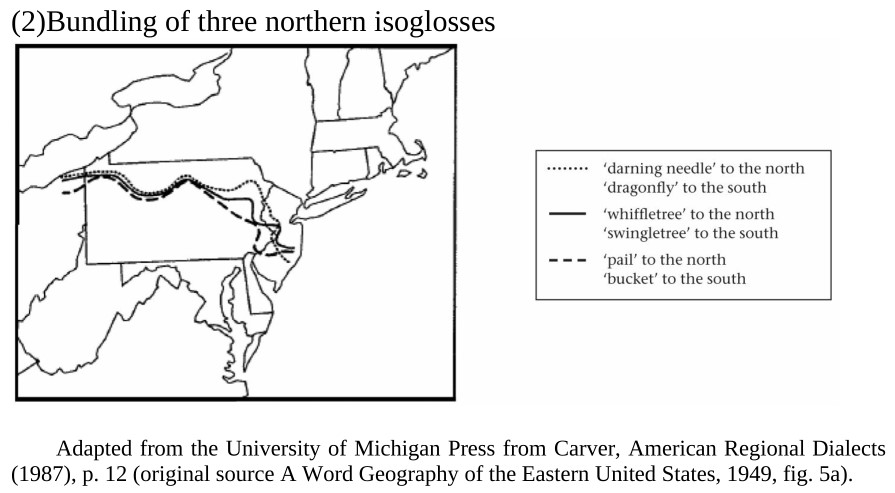
\includegraphics[scale=0.56]{pa_isogloss.jpg}
          \end{center}
        }
      \end{frame}

    \subsection{\subonethree}
      \begin{frame}{\subonethree}
        \begin{columns}
          \column{0.5\linewidth}
            \only<-2>{
              \begin{block}{Settlement patterns}
                \begin{itemize}
                  \item Colonists arrived from different parts of the UK
                  \item<2-> Colonists then spread out in different directions
                \end{itemize}
              \end{block}
            }
            \only<3>{
              \begin{block}{But it's not that simple}
                Colonists came into contact with:
                \begin{itemize}
                  \item Indian populations
                  \item Other European settlers
                  \begin{itemize}
                    \item French in LA, German in PA, Spanish in SW
                  \end{itemize}
                  \item African slaves who shaped the southern states
                \end{itemize}
              \end{block}
            }
            \only<4->{
              \begin{block}{And even less simple}
                African-Americans later migrated to the northern cities and further shaped the dialects there
              \end{block}
            }
          \column{0.5\linewidth}
            \only<1>{
              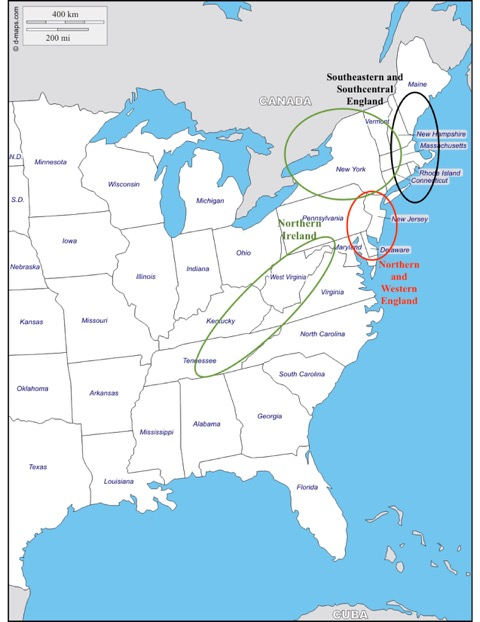
\includegraphics[scale=0.3]{eastern_usa1.jpg}
            }
            \only<2->{
              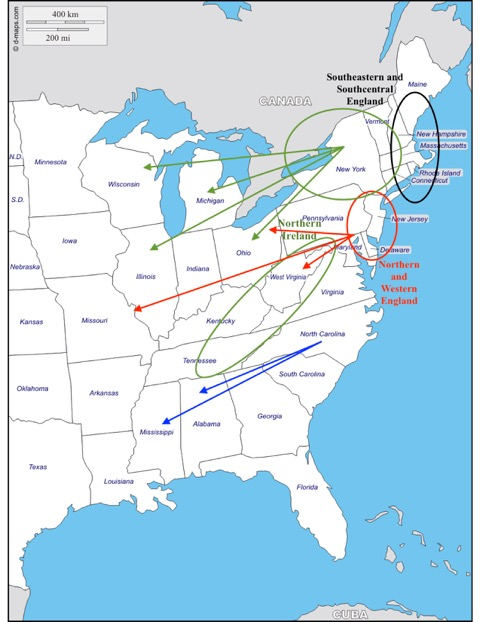
\includegraphics[scale=0.3]{eastern_usa2.jpg}
            }
        \end{columns}
      \end{frame}

      \begin{frame}[t]{\subonethree}
        \begin{center}
          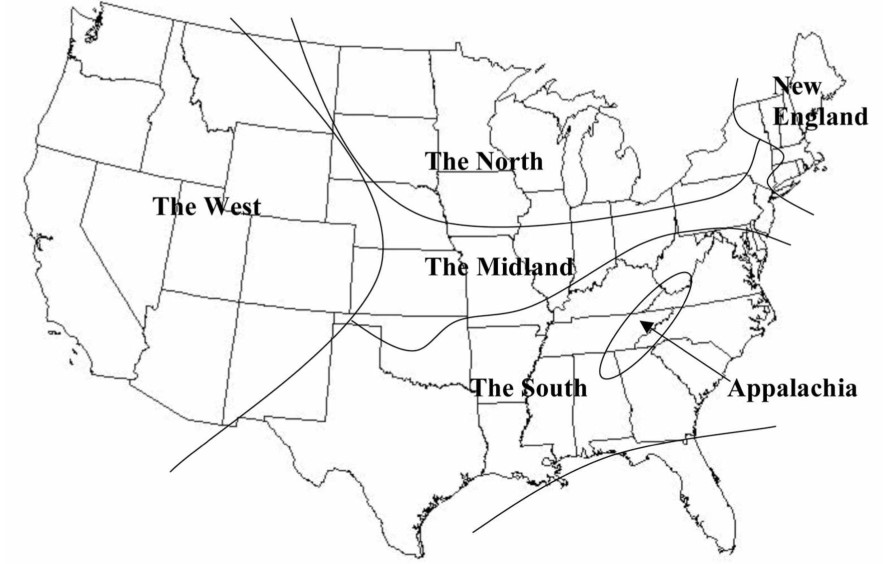
\includegraphics[scale=0.425]{supraregional_dialects.jpg}
        \end{center}
        \only<1>{
          \begin{block}{The resulting dialect regions}
            \begin{itemize}
              \item Homogenized a bit for the middle-class
              \item Stable for the working-class
            \end{itemize}
          \end{block}
        }
        \only<2->{
          \begin{block}{Doctrine of first effective settlement (Zelinsky, 1992)}
            The first group to settle an area has an outsized influence on the culture that develops there
          \end{block}
        }
      \end{frame}

    \subsection{\subonefour}
      \begin{frame}{\subonefour}
        \begin{columns}
          \column{0.5\linewidth}
            \begin{minipage}[t][0.6\textheight]{\linewidth}
              \begin{block}{Some features}
                \only<1>{
                \begin{itemize}
                  \item \href{https://youtu.be/9UoJ1-ZGb1w?t=59}{The northern cities vowel shift}
                  \item Gerunds where \lexi{to be} constructions are expected
                  \begin{enumerate}
                    \item The table needs cleaning
                    \item The table needs to be cleaned
                  \end{enumerate}
                \end{itemize}
                }
                \only<2>{
                \begin{itemize}
                  \item \lexi{By} where \lexi{at} is expected
                  \begin{enumerate}
                    \item I was by Sarah's house
                    \item I was at Sarah's house
                  \end{enumerate}
                  \item Lexical differences
                  \begin{itemize}
                    \item \lexi{sneaker}, \lexi{pop}, \lexi{roly-poly}
                  \end{itemize}
                \end{itemize}
                }
              \end{block}
            \end{minipage}
          \column{0.5\linewidth}
            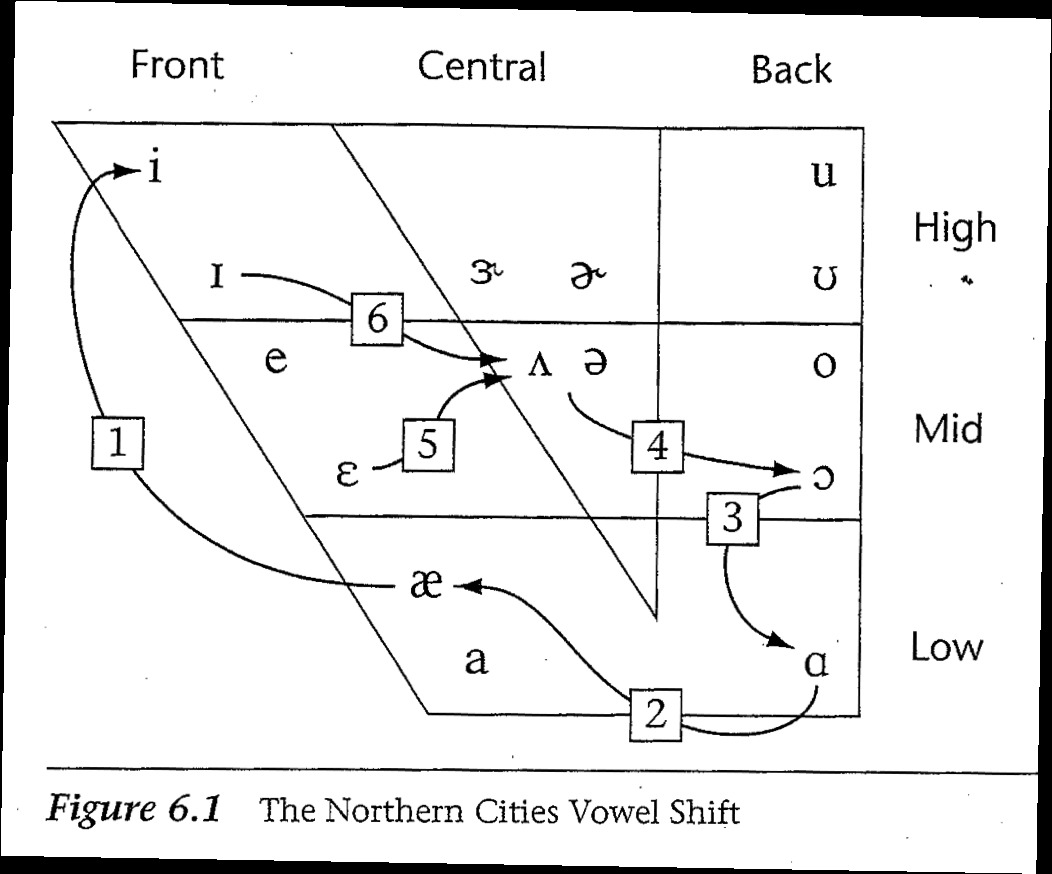
\includegraphics[scale=0.125]{northern_cities_shift.jpg}
        \end{columns}
      \end{frame}

      % "how do we end up with geographic variation"
        % Characteristics of the supra-regional dialects
          % New England


    \subsection{}
      \begin{frame}{}
        \begin{block}{Try these}
          % \textcite{dawson_language_2016}, chapter 10 exercises
        \end{block}
      \end{frame}

      \begin{frame}{References}
        % \printbibliography
      \end{frame}
\end{document}
